\chapter{Appendix}


\section{Code Repository}

The code for this project can be found on UCD School of Computer Science's internal GitLab server: \url{https://csgitlab.ucd.ie/rajitbanerjee/microservice-design-patterns}

\section{Supplementary Figures}

%%%%%%%%

\begin{figure}[H]
  \centering
  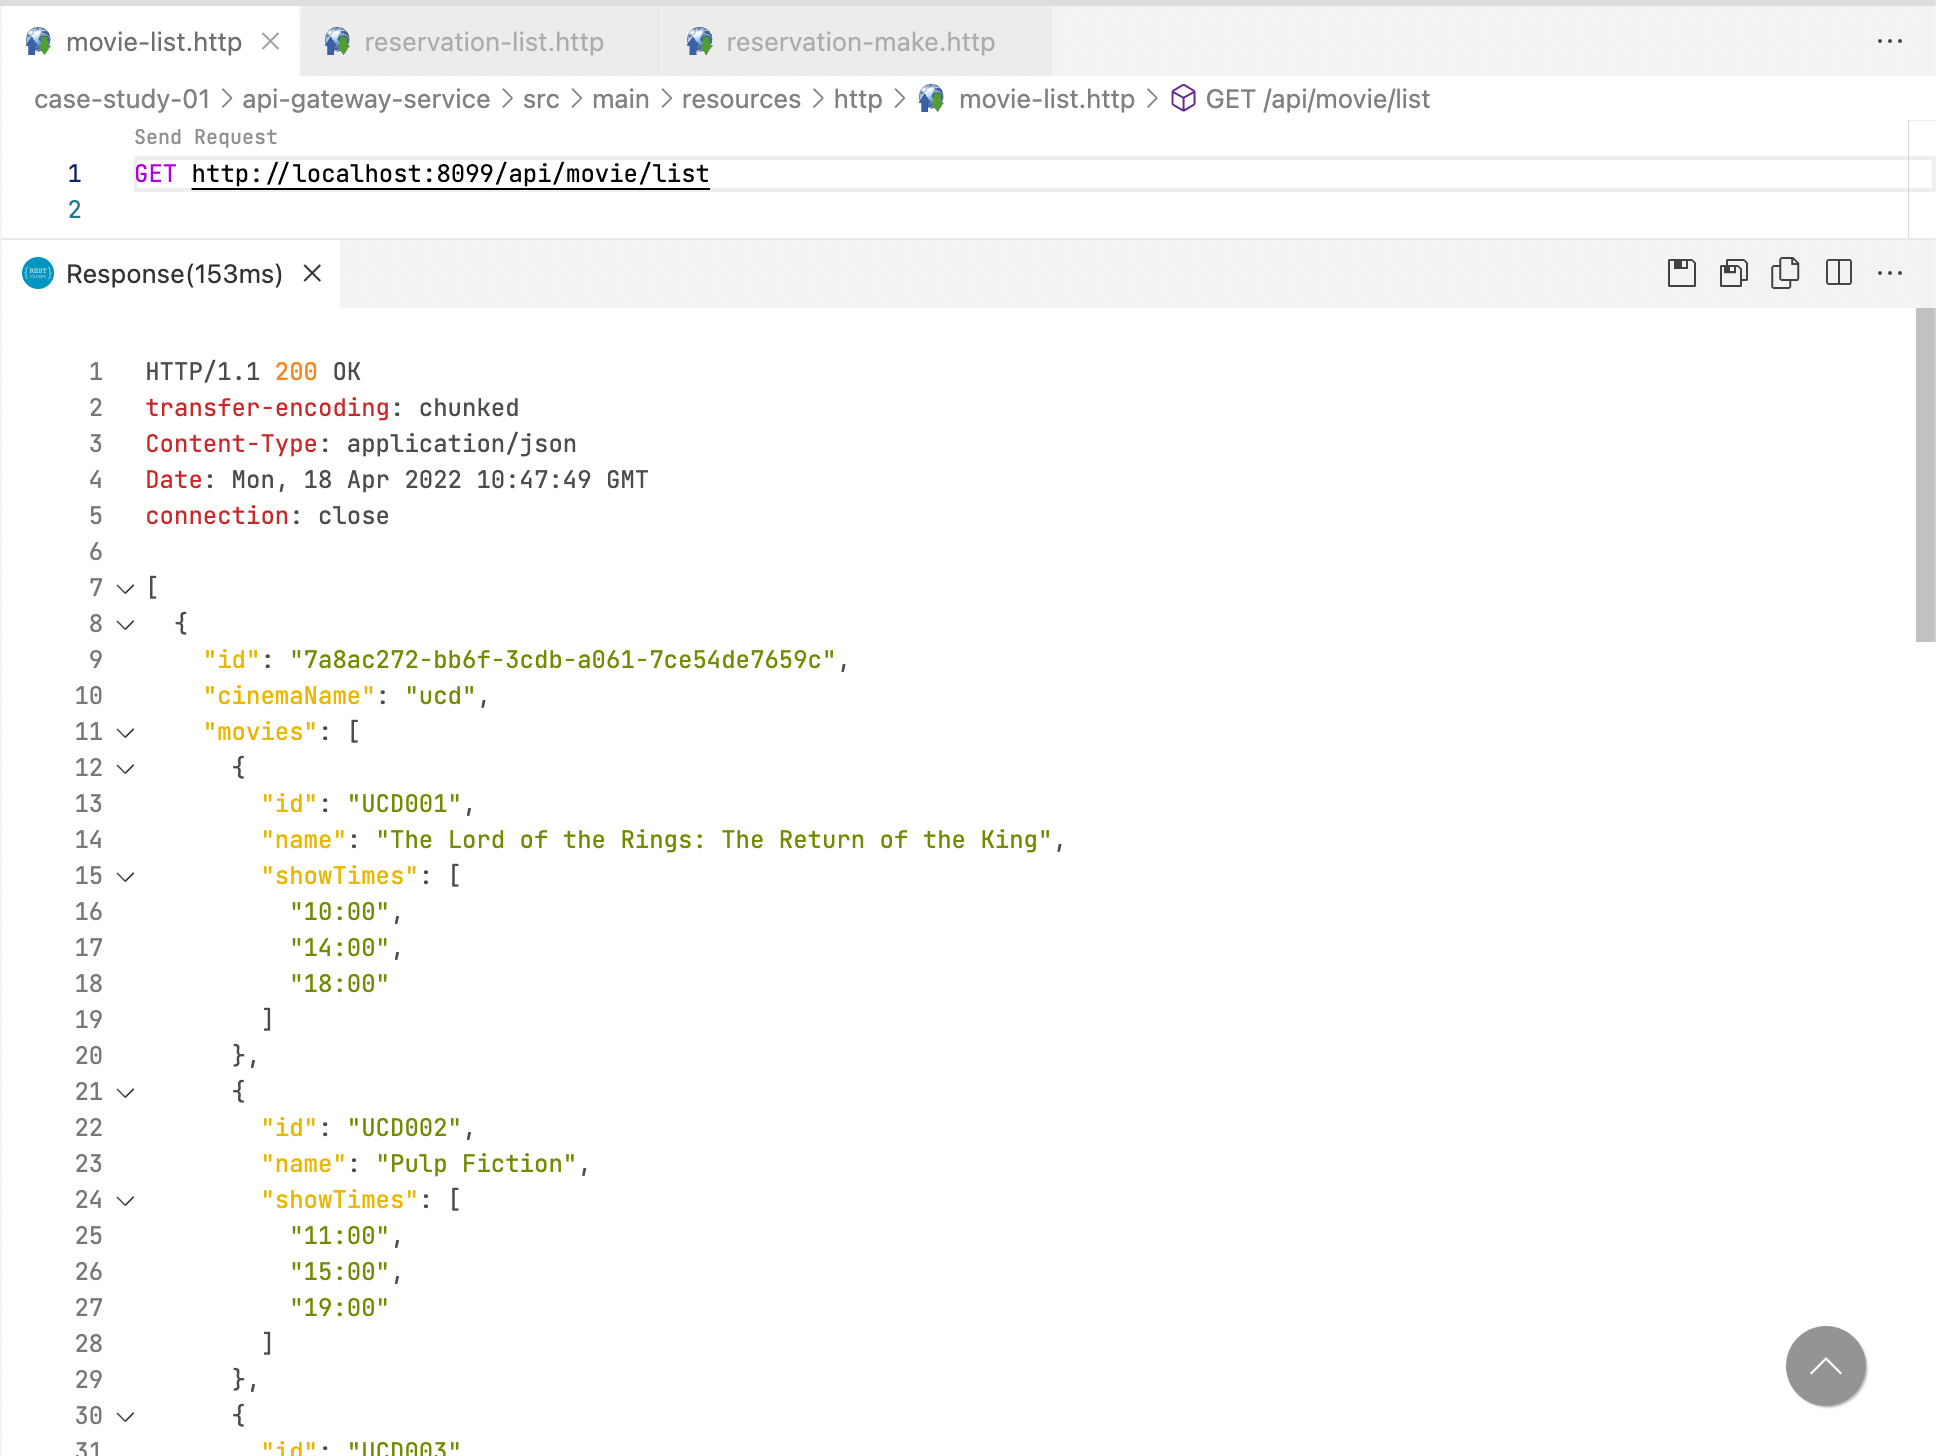
\includegraphics[width=1.0\linewidth]{./assets/images/case-studies/cs01-manual-1.png}
  \caption{Case Study 1 - manual API testing (listing all movie showtimes from various cinemas)}
  \label{fig:cs01-manual-1}
\end{figure}

\begin{figure}[H]
  \centering
  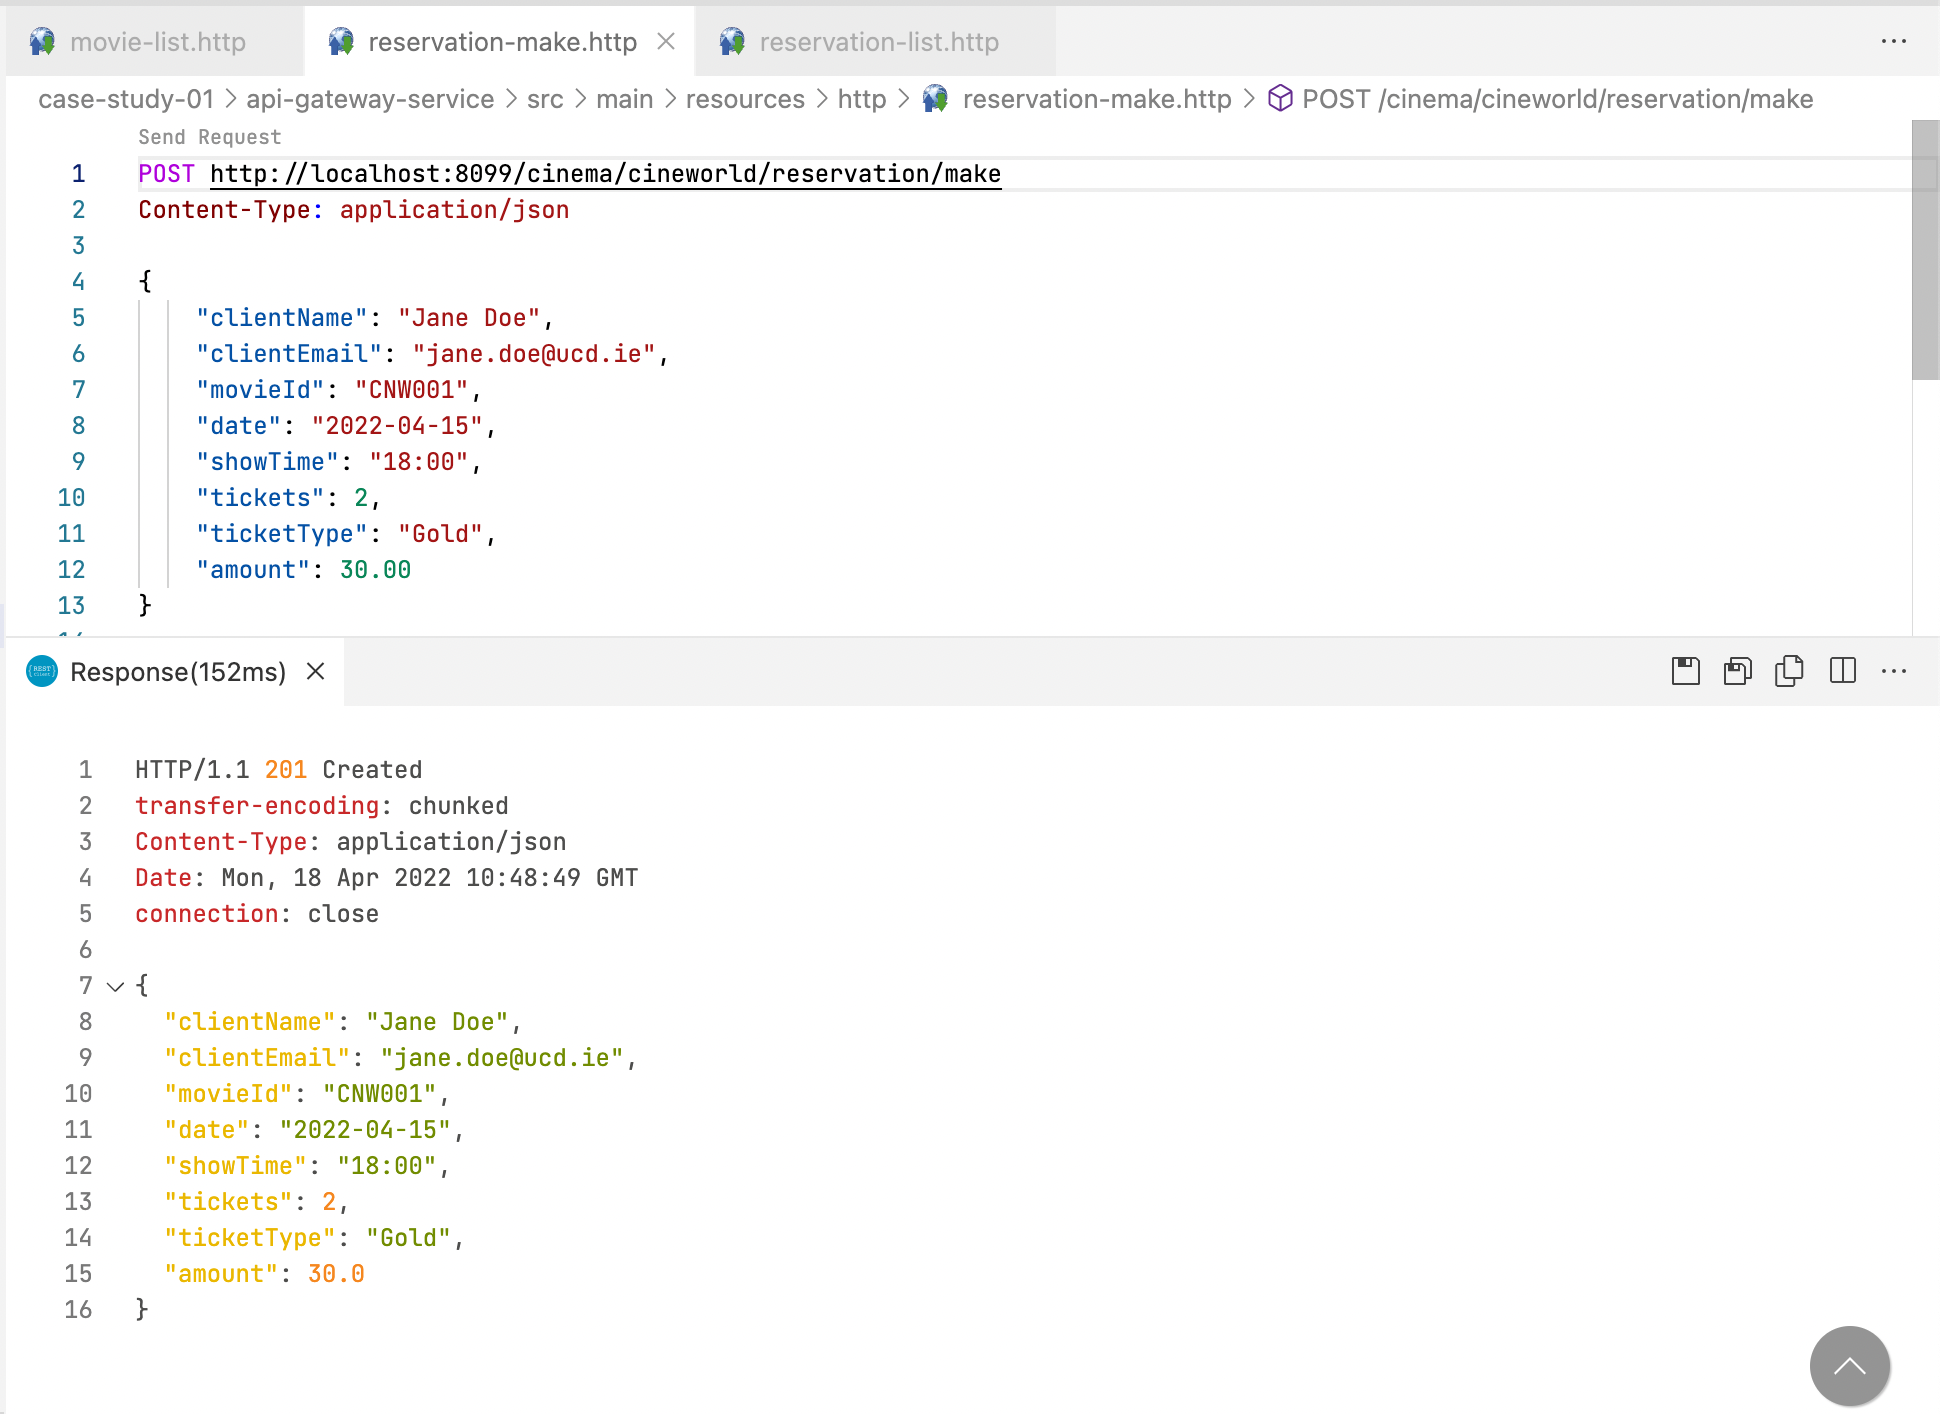
\includegraphics[width=1.0\linewidth]{./assets/images/case-studies/cs01-manual-2.png}
  \caption{Case Study 1 - manual API testing (making a reservation at Cineworld cinema)}
  \label{fig:cs01-manual-2}
\end{figure}

\begin{figure}[H]
  \centering
  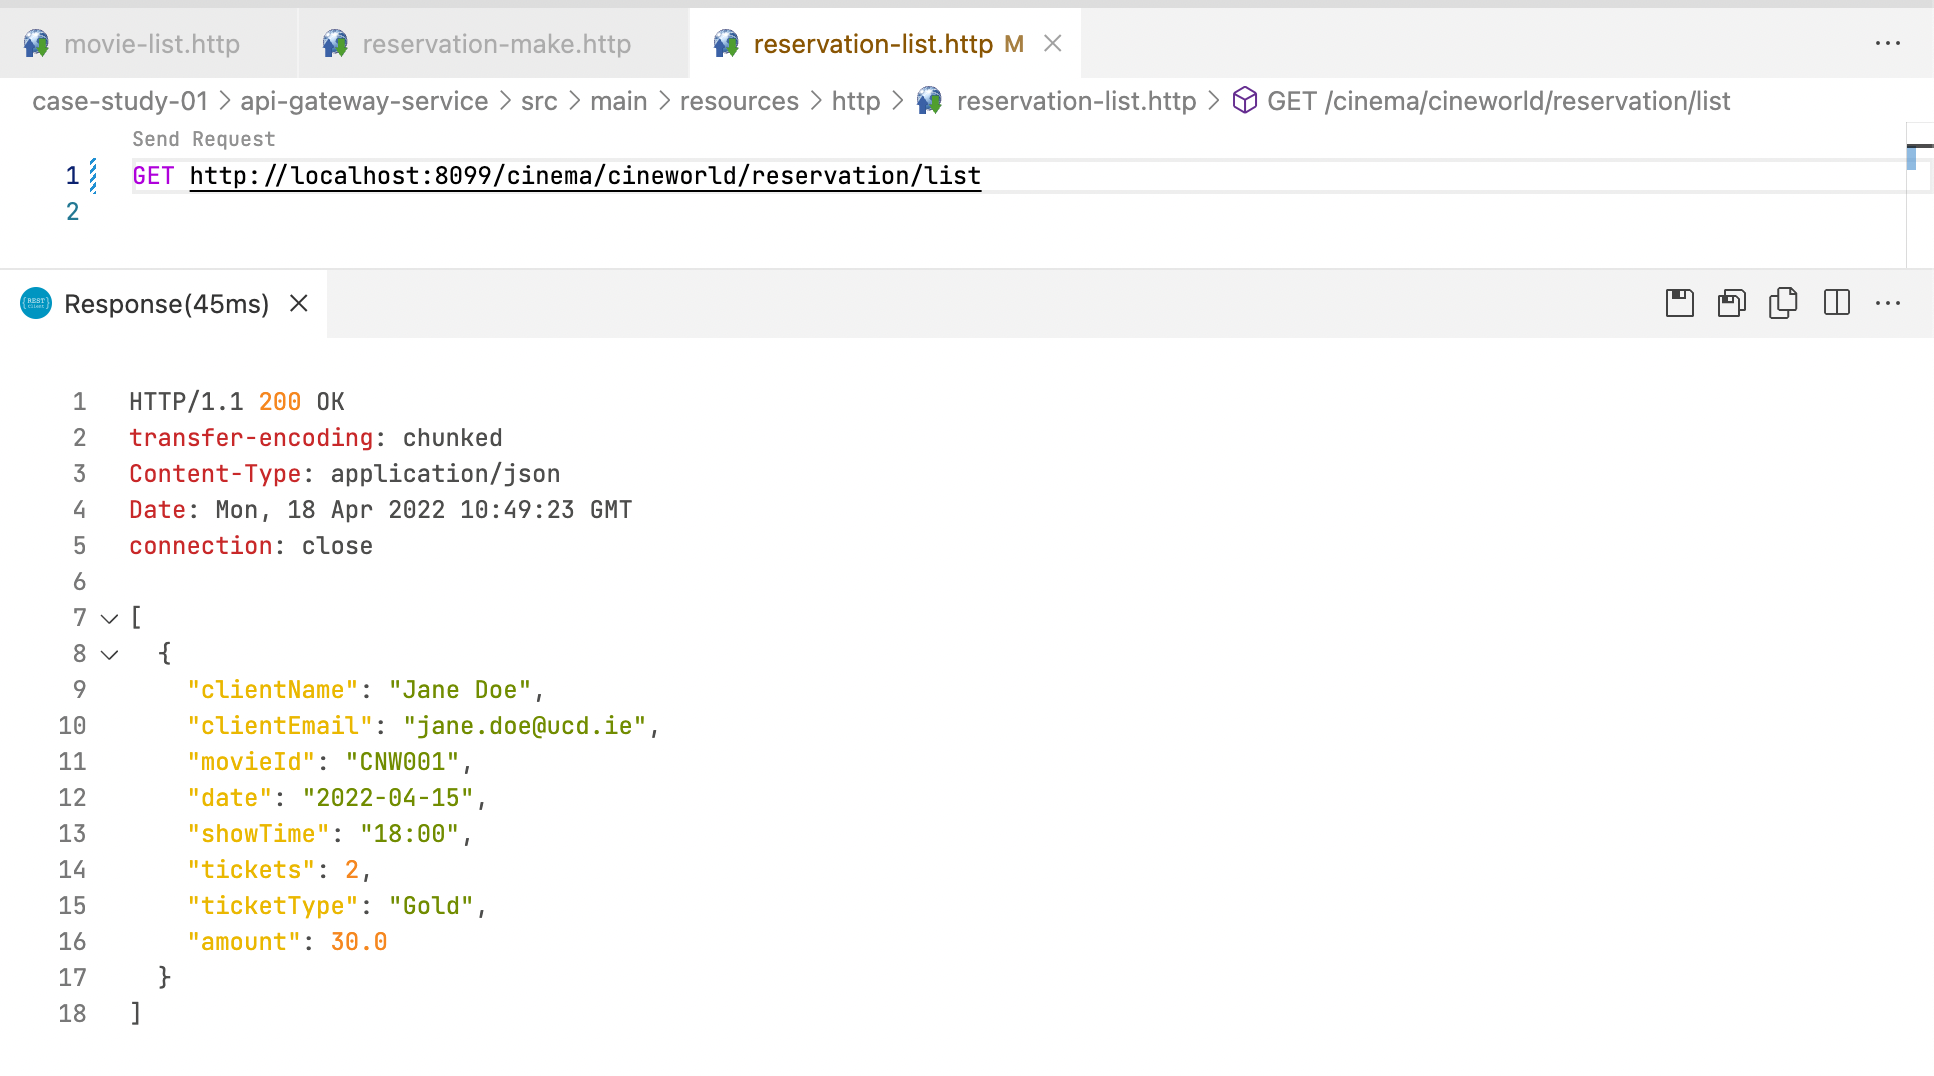
\includegraphics[width=1.0\linewidth]{./assets/images/case-studies/cs01-manual-3.png}
  \caption{Case Study 1 - manual API testing (listing all reservations at Cineworld to ensure the previous reservation was successful)}
  \label{fig:cs01-manual-3}
\end{figure}

\begin{figure}[H]
  \centering
  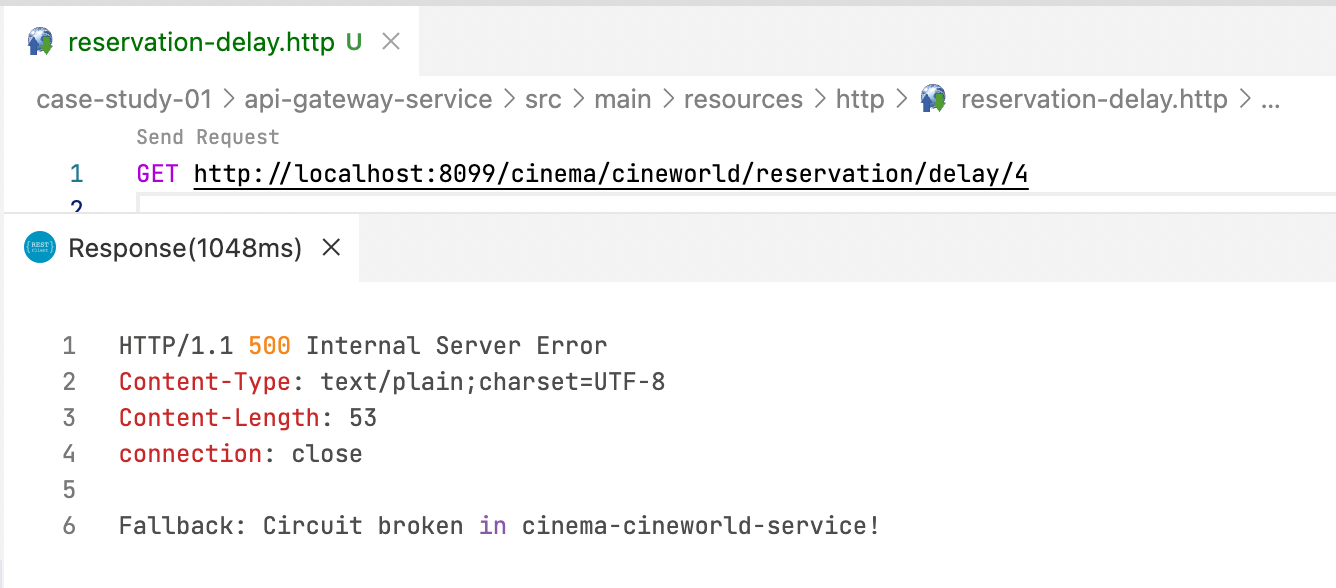
\includegraphics[width=1.0\linewidth]{./assets/images/case-studies/cs01-manual-4.png}
  \caption{Case Study 1 - manual API testing (reservation delay circuit breaker)}
  \label{fig:cs01-manual-4}
\end{figure}

%%%%%%%%

\begin{figure}[H]
  \centering
  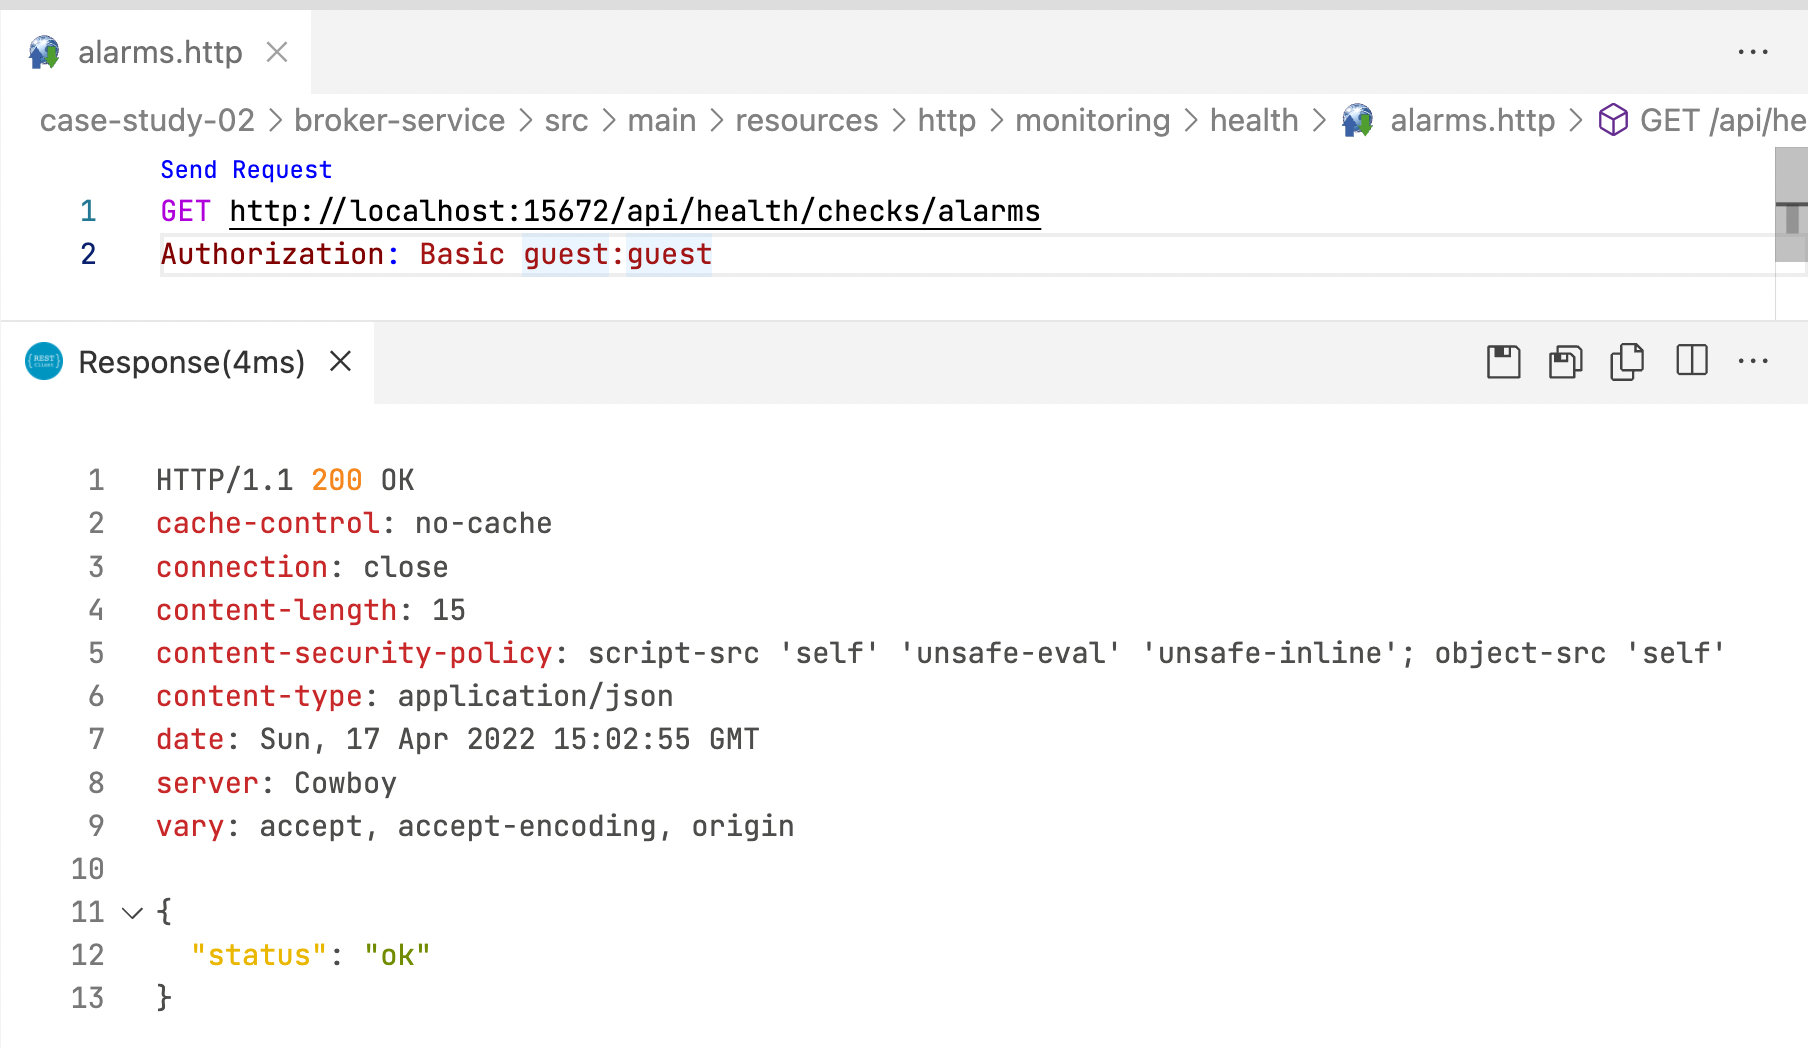
\includegraphics[width=1.0\linewidth]{./assets/images/case-studies/cs02-hc1.png}
  \caption{RabbitMQ health check - alarms}
  \label{fig:cs02-hc1}
\end{figure}

\begin{figure}[H]
  \centering
  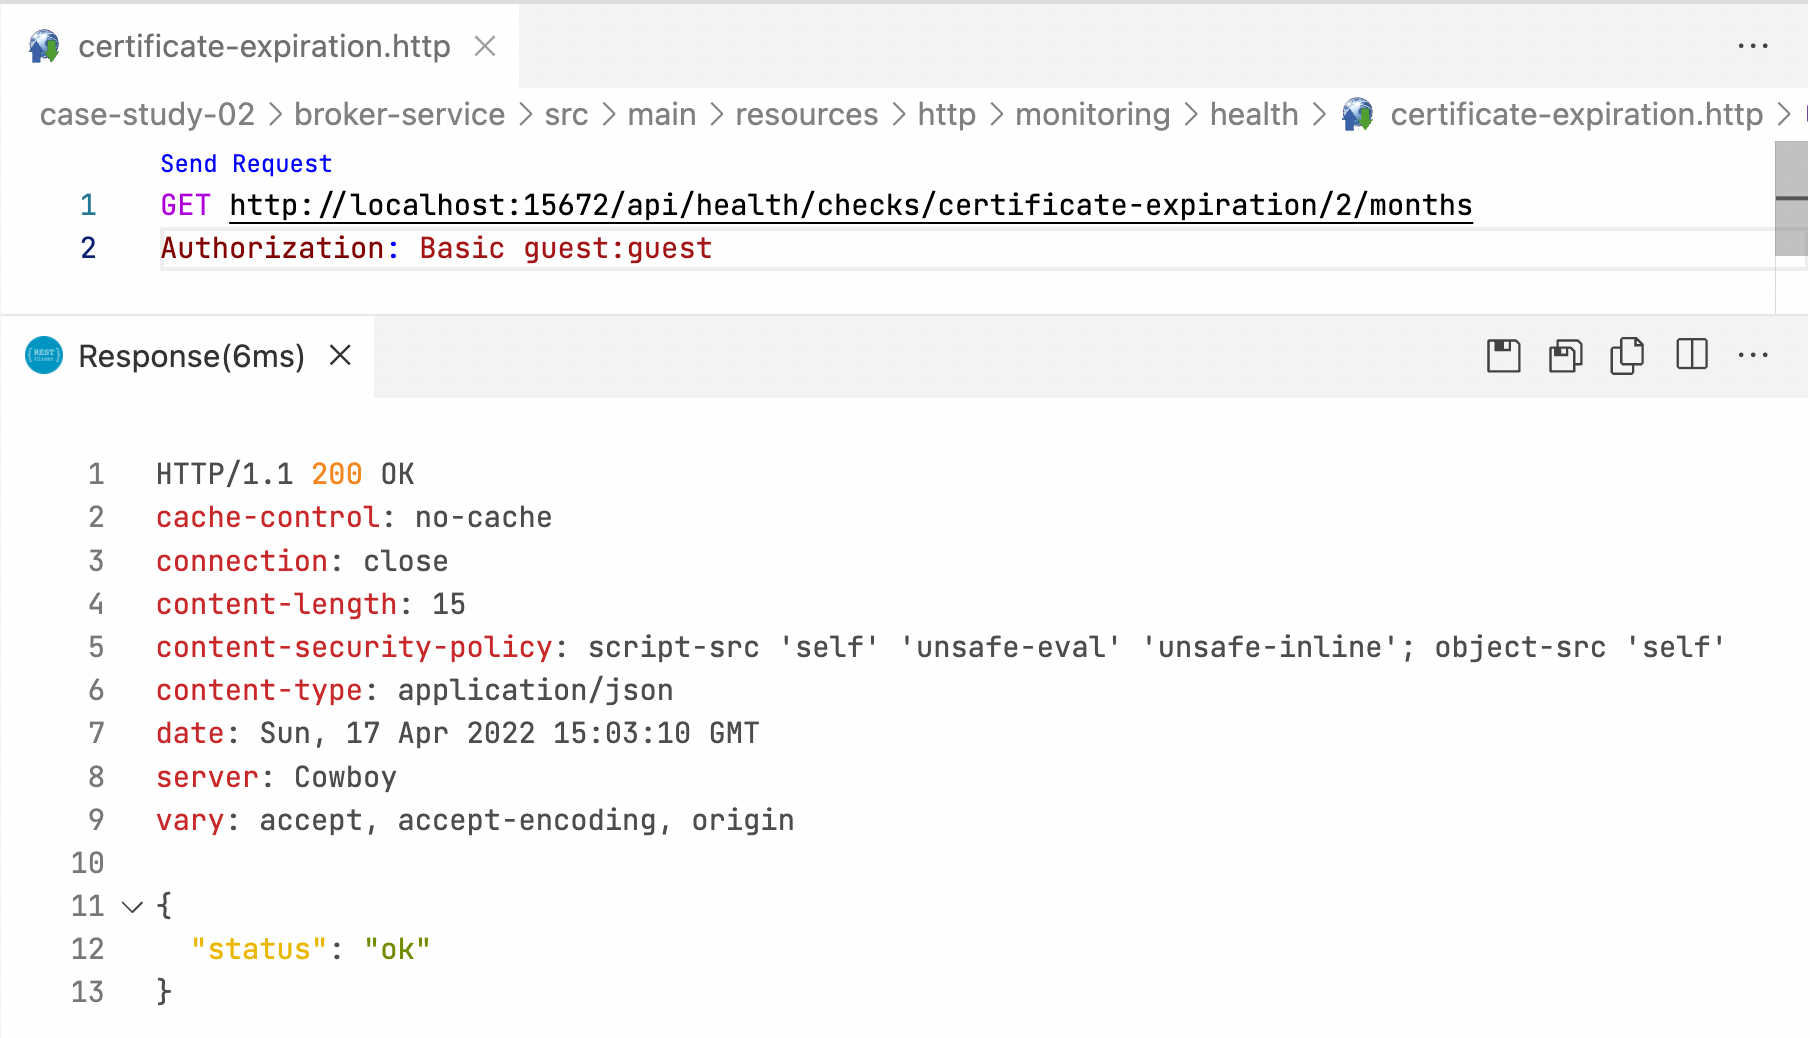
\includegraphics[width=1.0\linewidth]{./assets/images/case-studies/cs02-hc3.png}
  \caption{RabbitMQ health check - certificate expiration within a time unit (2 months)}
  \label{fig:cs02-hc3}
\end{figure}

\begin{figure}[H]
  \centering
  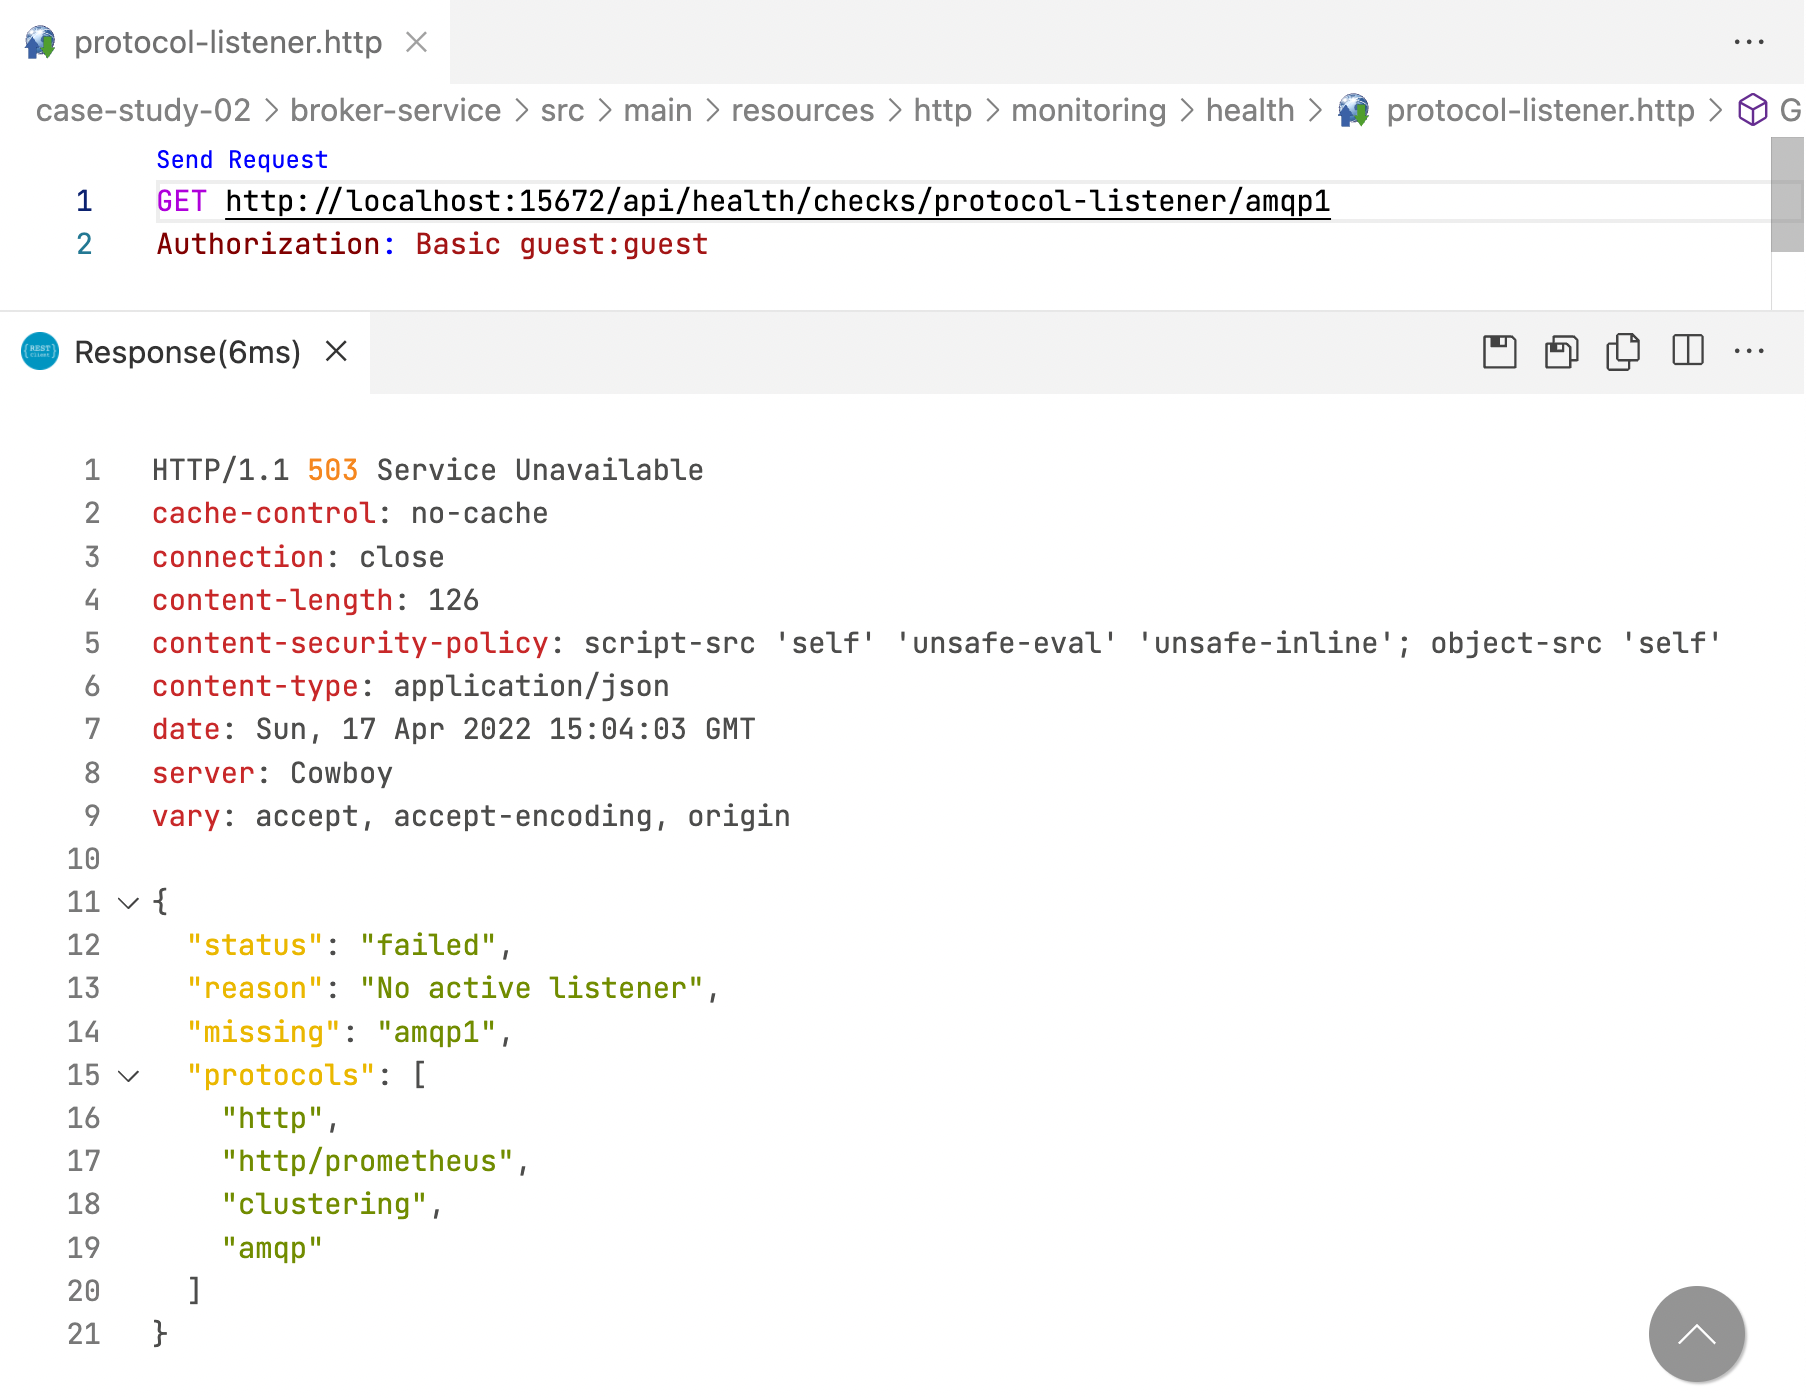
\includegraphics[width=1.0\linewidth]{./assets/images/case-studies/cs02-hc5.png}
  \caption{RabbitMQ health check - protocol listener}
  \label{fig:cs02-hc5}
\end{figure}

%%%%%%%%

\begin{figure}[H]
  \centering
  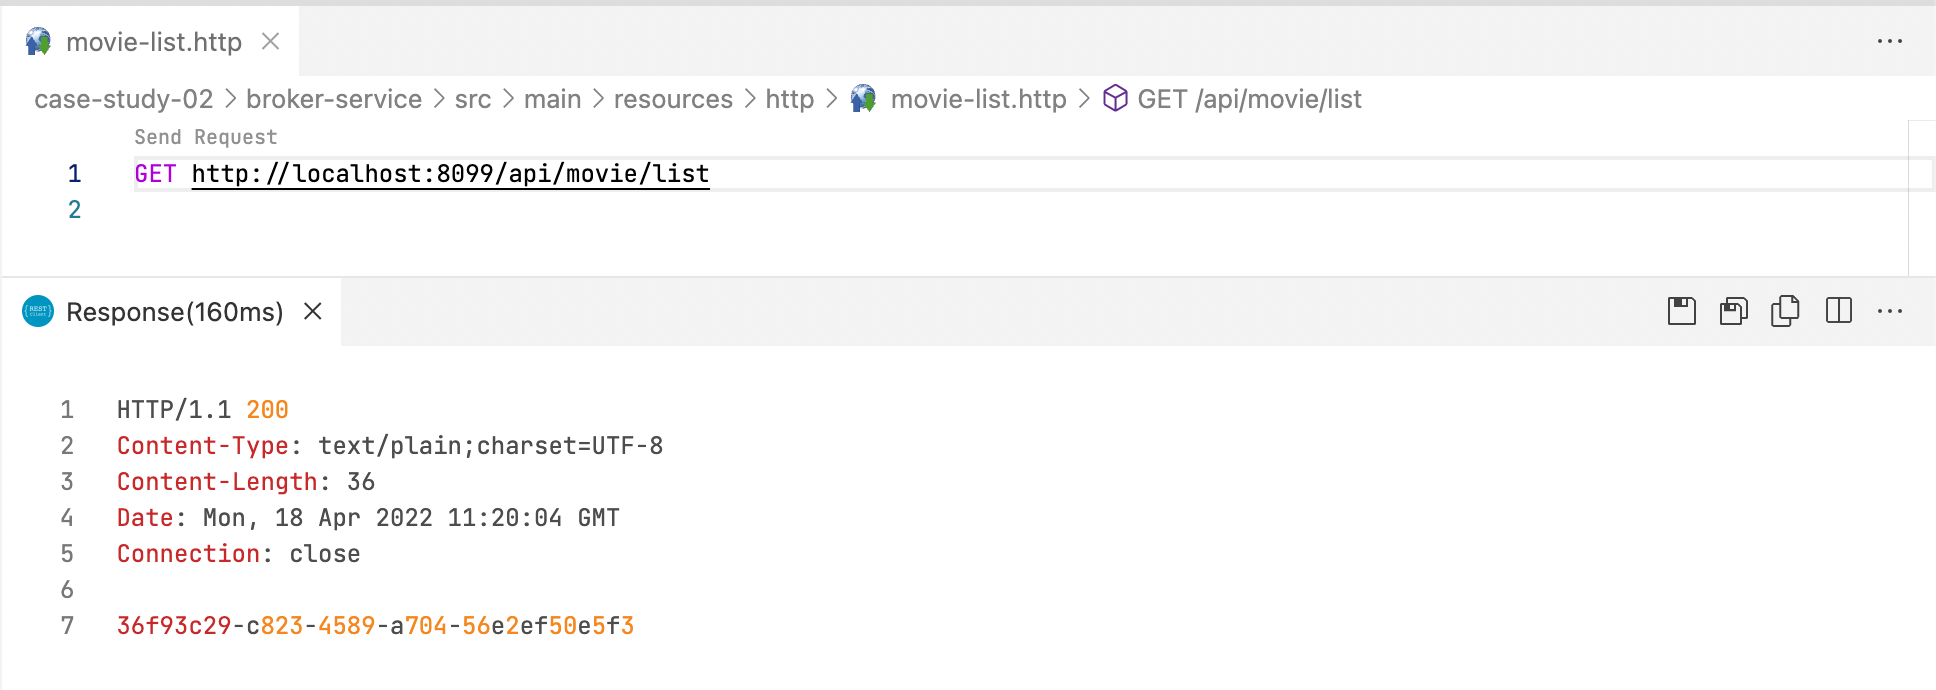
\includegraphics[width=1.0\linewidth]{./assets/images/case-studies/cs02-manual-1.png}
  \caption{Case Study 2 - manual API testing (send request to list all movies from various cinemas)}
  \label{fig:cs02-manual-1}
\end{figure}

\begin{figure}[H]
  \centering
  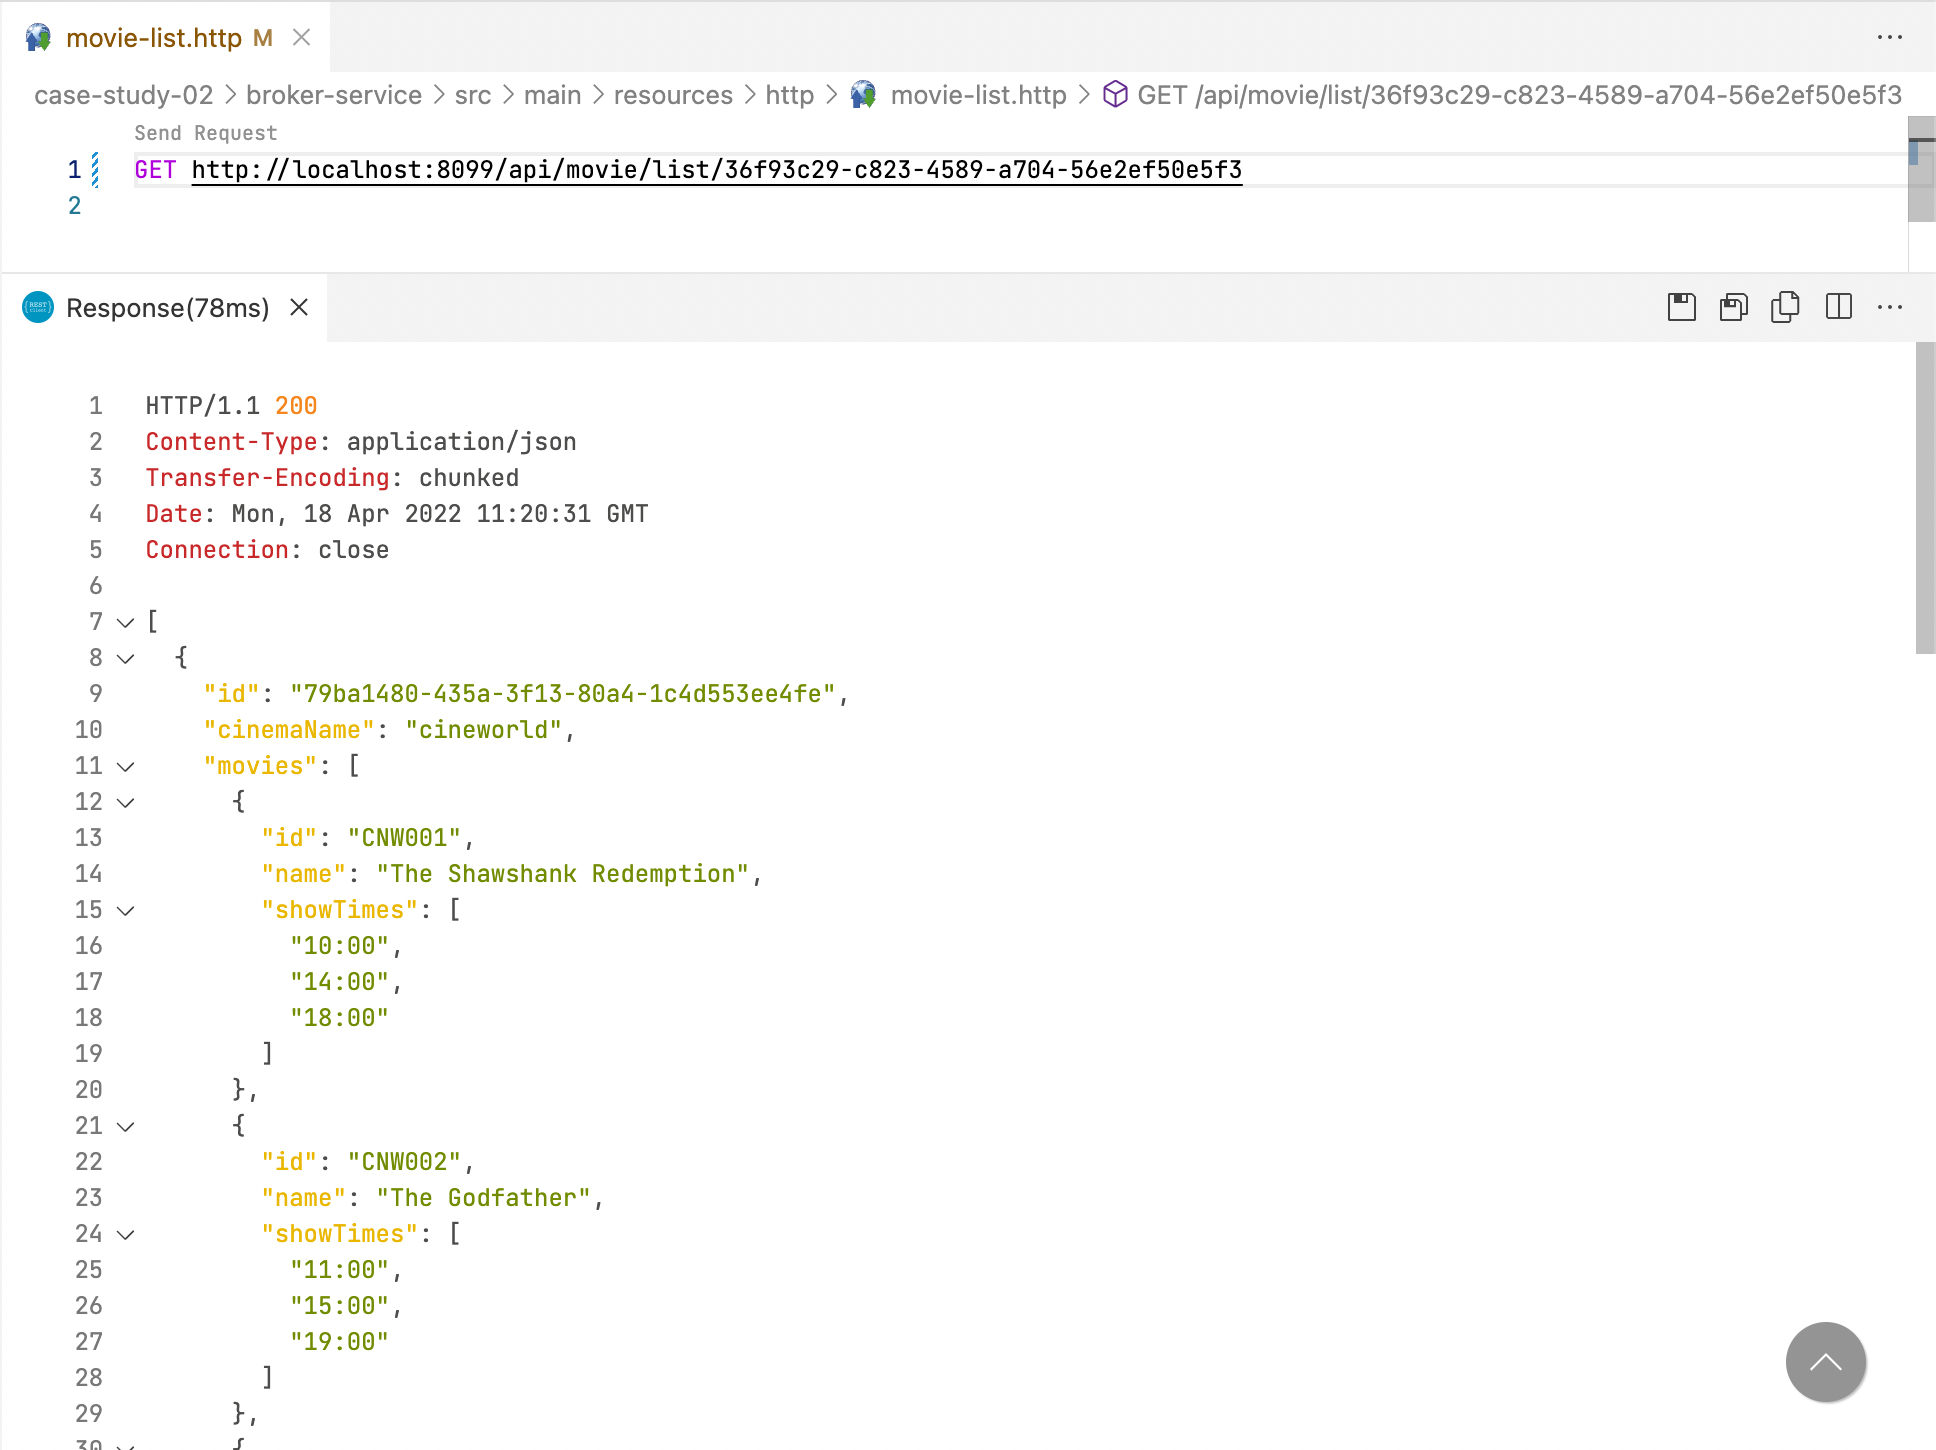
\includegraphics[width=1.0\linewidth]{./assets/images/case-studies/cs02-manual-2.png}
  \caption{Case Study 2 - manual API testing (receive response listing all movies)}
  \label{fig:cs02-manual-2}
\end{figure}

\begin{figure}[H]
  \centering
  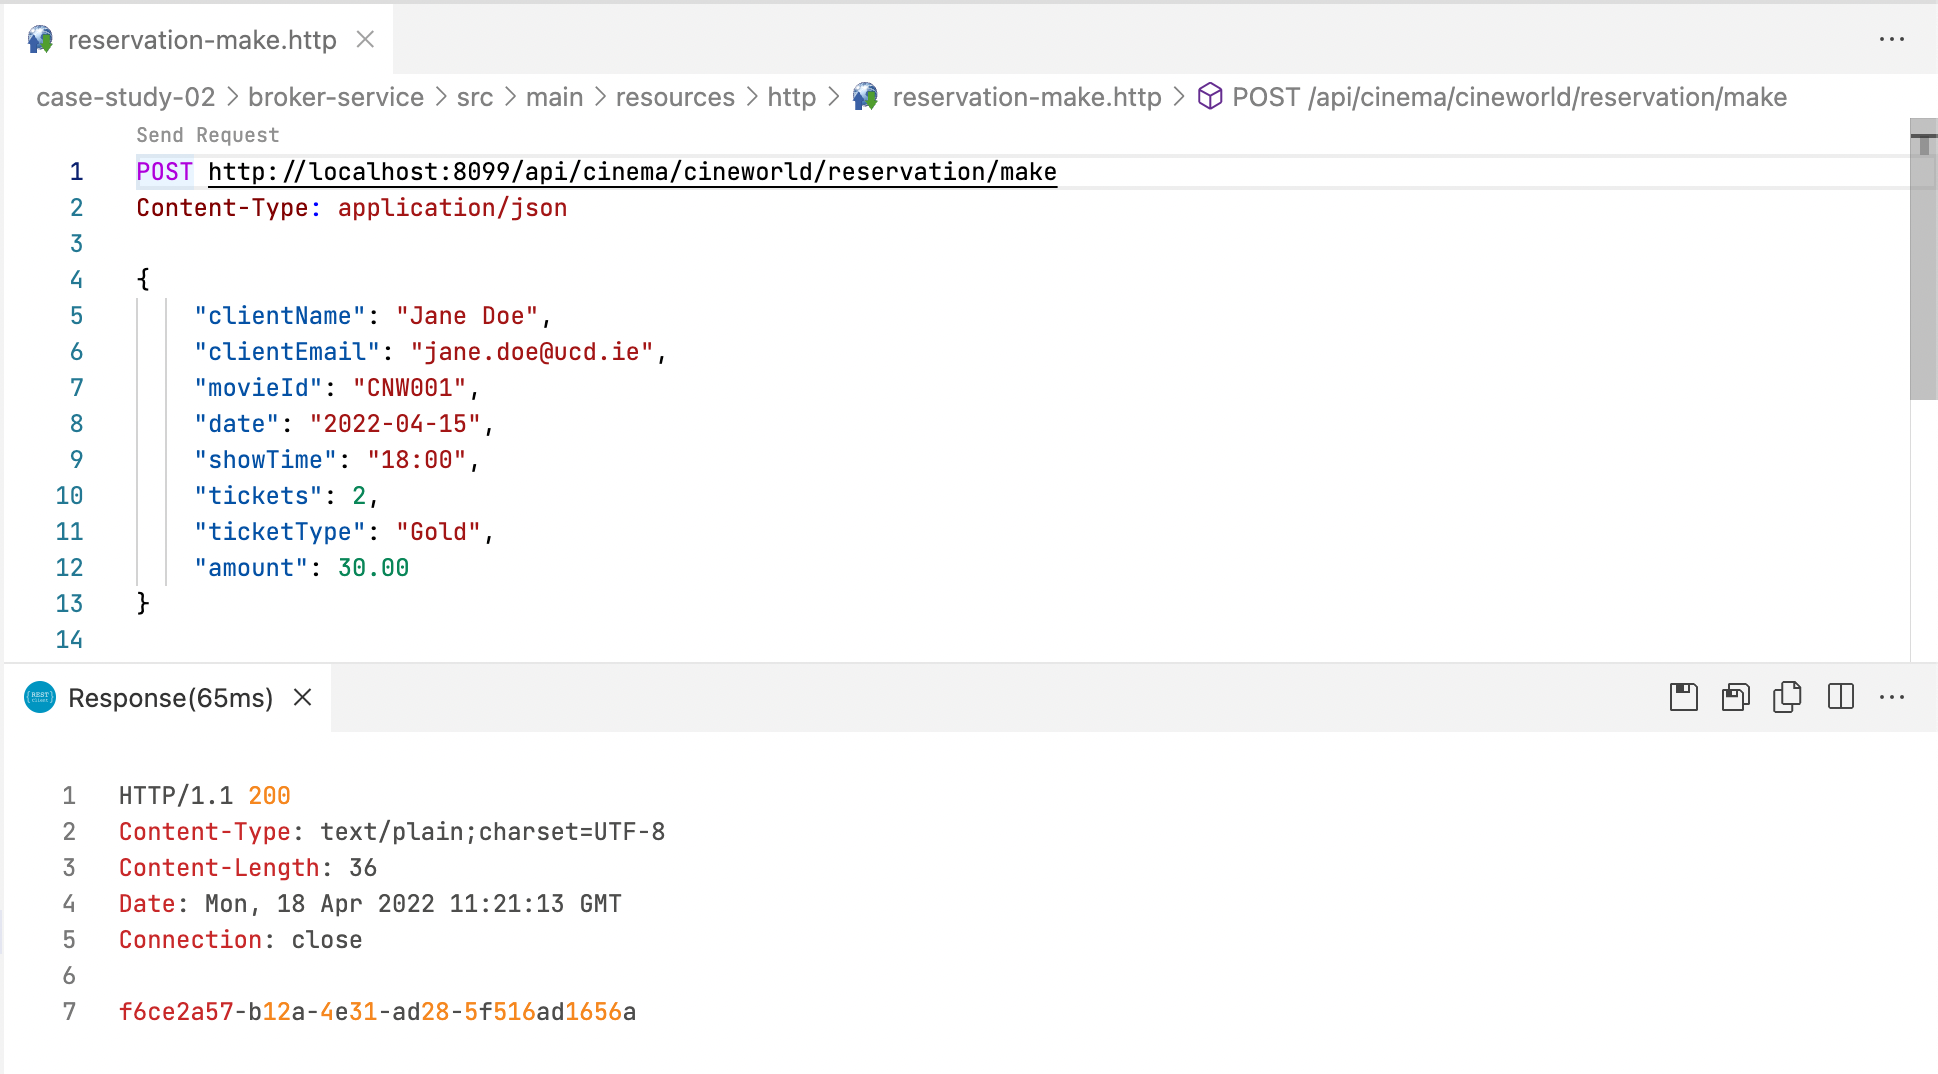
\includegraphics[width=1.0\linewidth]{./assets/images/case-studies/cs02-manual-3.png}
  \caption{Case Study 2 - manual API testing (send request to make a reservation at Cineworld cinema)}
  \label{fig:cs02-manual-3}
\end{figure}

\begin{figure}[H]
  \centering
  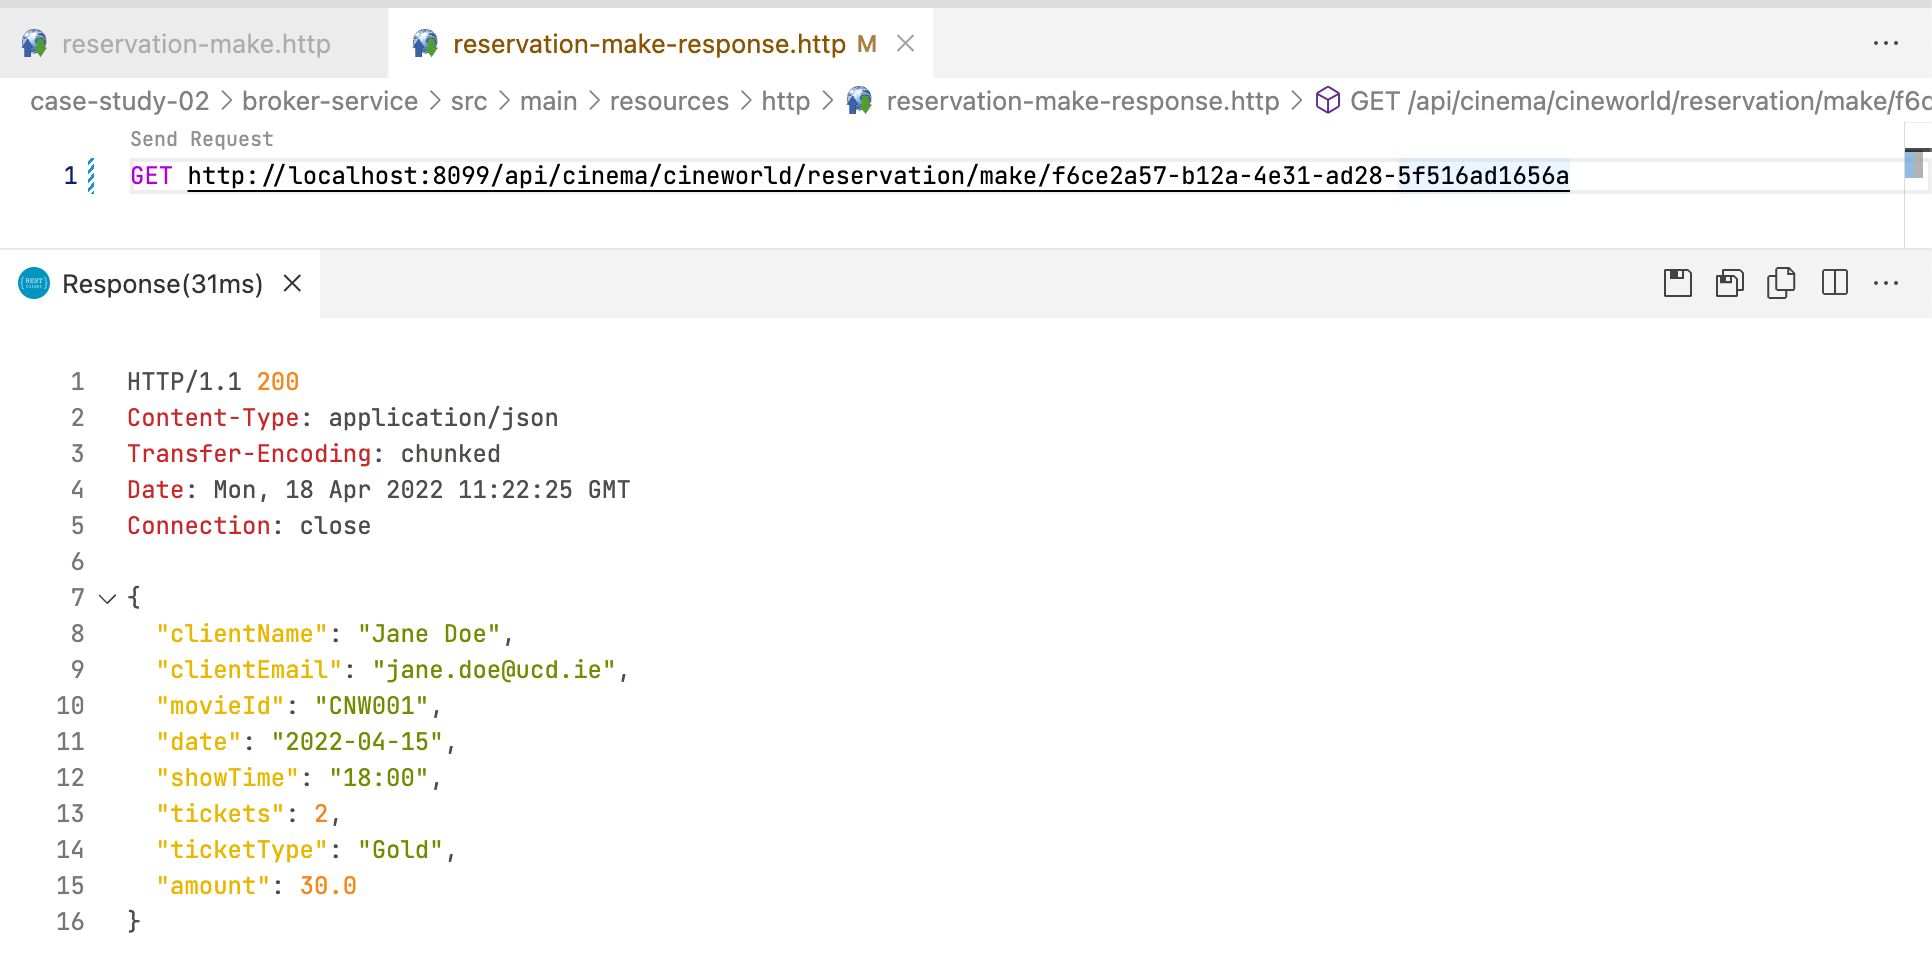
\includegraphics[width=1.0\linewidth]{./assets/images/case-studies/cs02-manual-4.png}
  \caption{Case Study 2 - manual API testing (receive response from Cineworld showing reservation)}
  \label{fig:cs02-manual-4}
\end{figure}

\begin{figure}[H]
  \centering
  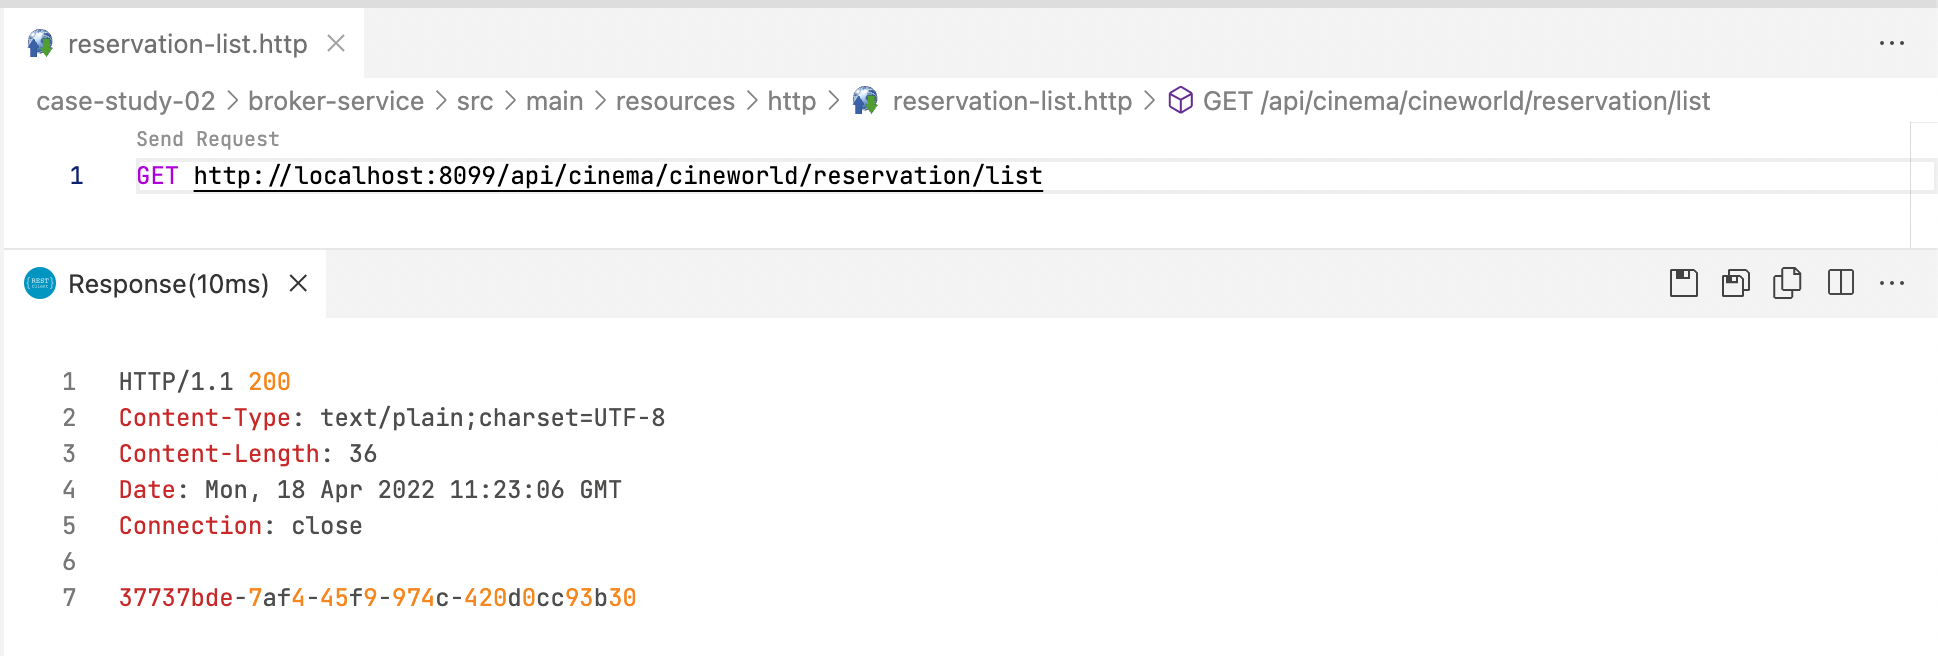
\includegraphics[width=1.0\linewidth]{./assets/images/case-studies/cs02-manual-5.png}
  \caption{Case Study 2 - manual API testing (send request to list all reservations at Cineworld)}
  \label{fig:cs02-manual-5}
\end{figure}

\begin{figure}[H]
  \centering
  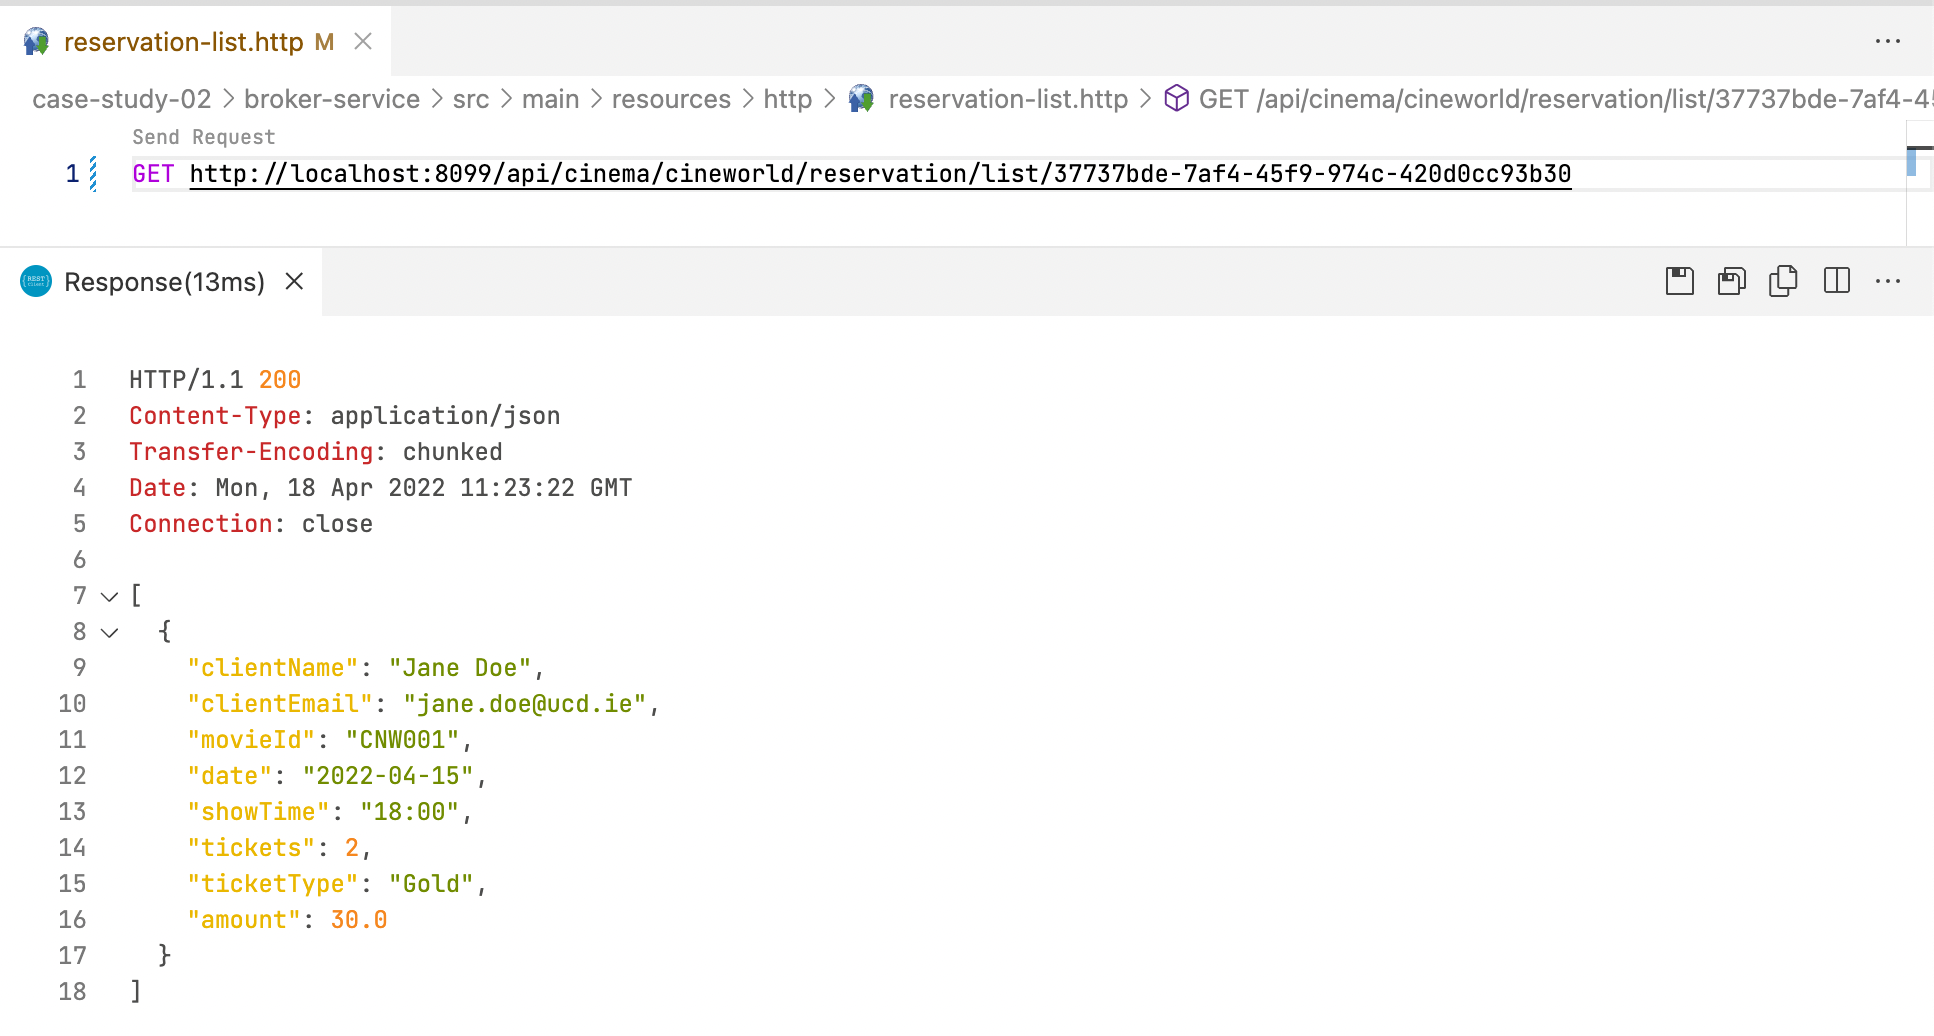
\includegraphics[width=1.0\linewidth]{./assets/images/case-studies/cs02-manual-6.png}
  \caption{Case Study 2 - manual API testing (receive response showing all of Cineworld's reservations)}
  \label{fig:cs02-manual-6}
\end{figure}

%%%%%%%%

\section{Initial Project Specification}

\subsection{Problem Statement}
Microservice architecture is a style of designing software systems to be highly maintainable, scalable, loosely-coupled and independently deployable. Moreover, each service is built to be self-contained and implement a single business capability. Design patterns in software engineering refer to any general, repeatable or reusable solution to recurring problems faced during the software design process. The aim of this project is to study the performance engineering practices associated with a number of \textit{microservice design patterns}, considering both qualitative and quantitative metrics to evaluate their benefits and shortcomings depending on the business requirement and use case. A non-exhaustive list of design patterns that could be explored is as follows:

\begin{itemize}
	\item API Gateway
	\item Asynchronous Messaging
	\item Chain of Responsibility
	\item Database or Shared Data
	\item Circuit Breaker
	\item Externalise Configuration
	\item Aggregator
	\item Branch
\end{itemize}

Employing some of the aforementioned design patterns, sufficiently complex simulations will be designed for the performance engineering experiments. The project will also look at some common issues in microservices, and how they compare with traditional monolithic architectures.

\subsection{Background}
Microservices have gained traction in recent years with the rise of Agile software development and a DevOps \cite{awsDevOps} approach. As software engineers migrate from monoliths to microservices, it is important to make appropriate choices for system design and avoid "anti-patterns". Although no one design pattern can be called the "best", the performance of systems can be optimised by following design patterns suited to the use case, with the right configuration of hardware resources.

\subsection{Related Work}
Due to their popularity, microservices have been written about extensively in books like \cite{richardson18}, \cite{kleppmann17}, \cite{newman14}. Articles such as \cite{md19}, \cite{md20}, \cite{sahiti20}, \cite{udantha19}, \cite{lewis14} discuss the intricacies of microservice architecture as well as the trade-offs between various common design patterns. In \cite{cully20}, the performance problems inherent to microservices are explored, with evaluations performed using a custom-built prototyping suite. Akbulut and Perros \cite{akbulut19} dive into the performance analysis aspect of microservices that is being proposed in this project, where they consider 3 different design patterns.

\subsection{Datasets}
Any data that is to be used or analysed in this project will be generated during the course of experiments. There are no dependencies on additional datasets.

\subsection{Resources Required}
A non-exhaustive list of resources is specified below, following preliminary needs assessment.

\begin{itemize}
	\item Languages/Frameworks: Java, Spring Boot, Python
	\item Tools: Git, Docker, Apache JMeter
	\item Database: MongoDB
	\item Compute: Linux server maintained by the UCD School of Computer Science
\end{itemize}



%%%%%%%%

\chapter{Project Work Plan}

\begin{figure}[h]
	\centering
	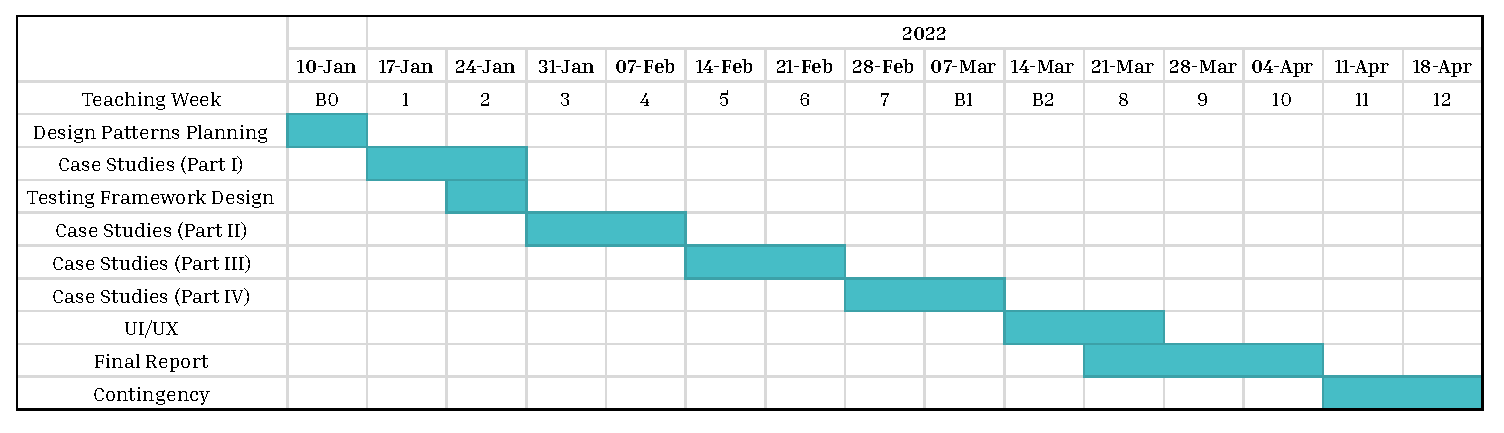
\includegraphics[width=1.0\linewidth]{./assets/images/work-plan-gantt.pdf}
	\caption{Gantt chart for project timeline}
	\label{fig:work-plan-gantt}
\end{figure}

\begin{itemize}
	\item \textbf{Design Patterns Planning (1 week)}: The initial planning here is of particular significance and will decide the direction and pace of the project's implementation phase. Various microservice design patterns will be considered to select a few important patterns which can be easily demonstrated using simulations, and then performance tested.

	\item \textbf{Testing Framework Design (1 week)}: Designing a simple testing framework (e.g. load testing plans) during the first case study will facilitate the adoption of similar strategies for subsequent case studies. 

	\item \textbf{Case Studies (Parts I, II, III, IV) (8 weeks)}: These case studies will form the bulk of the project, and will be split into four parts for convenience, each comprising a set of related design patterns (each group of case studies will possibly address 2-3 patterns). The majority of effort required here will be concerned with the back-end development of dummy microservice-based systems using containers (Docker). Evaluation, both qualitative and quantitative, is well integrated with the implementation phase of the project, since performance analysis/testing will be carried out in tandem with the case study experiments. Different configurations used during performance testing will facilitate the discussion around suitability and aptness of a number of microservice design patterns.

	\item \textbf{UI/UX (2 weeks)}: A simple web user interface will be designed to visualise the results of performance testing conducted for microservices during the different case studies, and also provide a cost-benefit analysis of the design patterns under investigation.

	\item \textbf{Final Report (3 weeks)}: Although the core parts of the report should be written as progress is made with tasks, a dedicated period is set aside for refinement and completion.

	\item \textbf{Contingency (2 weeks)}: Time set aside to be used only in the event of unforeseen issues or challenges.
\end{itemize}



